\section{Introduction}

\subsection{Project Background}
The development of RAVEN started in 2012 when, within the Nuclear Energy
Advanced Modeling and Simulation (NEAMS) program~\cite{neams}, the need of a modern
risk evaluation framework arose.
RAVEN's principal assignment is to provide the necessary software and algorithms
in order to employ the concepts developed by the Risk Informed Safety Margin
Characterization (RISMC) Pathway.
RISMC is one of the pathways defined within the Light Water Reactor
Sustainability (LWRS) program~\cite{lwrs}.

The goal of the RISMC approach is  the identification not only of the frequency of an
event which can potentially lead to system failure, but also the proximity (or lack
thereof) to key safety-related events: the safety margin.
Hence, the approach is interested in identifying and increasing the safety
margins related to those events.
A safety margin is a numerical value quantifying the probability that a safety
metric (e.g. peak pressure in a pipe) is exceeded under certain conditions.
% Conclusion
Most of the capabilities, implemented having Reactor Excursion and Leak Analysis Program v.7
(RELAP-7) as a principal focus, are
easily deployable to other system codes.
%
For this reason, several side activates have been employed (e.g.  RELAP5-3D~\cite{RELAP5userManual}, any Multiphysics Object Oriented
Simulation Environment-based App, etc.)
or are currently ongoing for coupling RAVEN with several different software.
%

\subsection{Acquiring and Installing RAVEN}
RAVEN is supported on three separate computing platforms: Linux, OSX (Apple Macintosh), and Microsoft Windows.
Currently, RAVEN is open-source and downloadable from RAVEN GitHub repository: \url{https://github.com/idaholab/raven}.
New users should visit \url{https://github.com/idaholab/raven/wiki} or refer to the user manual ~\cite{RAVENuserManual}
to get started with RAVEN. This typically involves the following steps:
\begin{itemize}
  \item \textit{Download RAVEN}
    \\ You can download the source code of RAVEN from \url{https://github.com/idaholab/raven}.
  \item \textit{Install RAVEN dependencies}
    \\ Instructions are available from \url{https://github.com/idaholab/raven/wiki}, or the user manual ~\cite{RAVENuserManual}.
  \item \textit{Install RAVEN}
    \\ Instructions are available from \url{https://github.com/idaholab/raven/wiki}, or the user manual ~\cite{RAVENuserManual}.
  \item \textit{Run RAVEN}
    \\ If RAVEN is installed successfully, please run the regression tests to verify your installation:
    \begin{lstlisting}[language=bash]
      ./run_tests
    \end{lstlisting}
    Normally there are skipped tests because either some of the codes are not available, or some of the test are not
    currently working. The output will explain why each is skipped. If all the tests pass, you are ready to run RAVEN.
    Now, open a terminal and use the following command (replace \texttt{<inputFileName.xml>} with your
    RAVEN input file):
    \begin{lstlisting}[language=bash]
      raven_framework <inputFileName.xml>
    \end{lstlisting}
    where the \texttt{raven\_framework} script can be found in the RAVEN folder. Alternatively, the \texttt{Driver.py} script
    contained in the folder ``\texttt{raven/framework}'' can be directly used:
    \begin{lstlisting}[language=bash]
      python raven/framework/Driver.py <inputFileName.xml>
    \end{lstlisting}
  \item \textit{Participate in RAVEN user communities}
    \\ Join RAVEN mail lists to get help and updates of RAVEN: \url{https://groups.google.com/forum/#!forum/inl-raven-users}.
\end{itemize}

\subsection{User Guide Formats}
In order to highlight some parts of the user guide having a particular meaning (input structure, examples, terminal commands, etc.), specific formats have been used. This section provides the formats with a specific meaning:
\begin{itemize}
\item \textbf{\textit{Python Coding:}}
\begin{lstlisting}[language=python]
class AClass():
  def aMethodImplementation(self):
    pass
\end{lstlisting}
\item \textbf{\textit{RAVEN XML input example:}}
\begin{lstlisting}[style=XML,morekeywords={anAttribute}]
<MainXMLBlock>
  ...
  <aXMLnode name='anObjectName' anAttribute='aValue'>
     <aSubNode>body</aSubNode>
  </aXMLnode>
  <!-- This is  commented block -->
  ...
</MainXMLBlock>
\end{lstlisting}
\item \textbf{\textit{Bash Commands:}}
\begin{lstlisting}[language=bash]
cd trunk/raven/
./raven_libs_script.sh
cd ../../
\end{lstlisting}
\end{itemize}



\subsection{Capabilities of RAVEN}
% High-level RAVEN description
RAVEN~\cite{alfonsiMC} ~\cite{alfonsiPSA}~\cite{RAVENFY13}~\cite{ESREL2014} is a software framework that allows the user to perform parametric and stochastic
analysis based on the response of complex system codes.
The initial development was designed to provide dynamic probabilistic risk analysis
capabilities (DPRA) to the thermal-hydraulic code RELAP-7~\cite{relap7FY12}, currently under development
at Idaho National Laboratory (INL).
Now, RAVEN is not only a framework to perform DPRA but it is a flexible and
multi-purpose uncertainty quantification, regression analysis, probabilistic risk assessment, data analysis and
model optimization platform. Depending on the tasks to be accomplished and on the probabilistic characterization
of the problem, RAVEN perturbs (e.g., Monte-Carlo, Latin hypercube, reliability surface search) the response of
the system under consideration by altering its own parameters. The system is modeled by third party software
(e.g., RELAP5-3D, MAAP5, BISON, etc.) and accessible to RAVEN either directly (software coupling) or indirectly
(via input/output files). The data generated by the sampling process is analyzed using classical statistical
and more advanced data mining approaches. RAVEN also manages the parallel dispatching
(i.e. both on desktop/workstation and large High Performance Computing machines) of the software representing the
physical model. RAVEN heavily relies on artificial intelligence algorithms to construct surrogate models of
complex physical systems in order to perform uncertainty quantification, reliability analysis (limit state surface)
and parametric studies.

The main capabilities of RAVEN, with brief descriptions, are summarized here, or one can check the Figure.~\ref{fig:ravenCap}.
These capabilities may be used on their own or as building blocks to construct the sought workflow. In addition, RAVEN also provides some more sophisticated
\textbf{Ensemble algorithms} such as \textbf{EnsembleForward}, \textbf{EnsembleModel} to combine the existing
capabilites.

\begin{figure}[h!]
  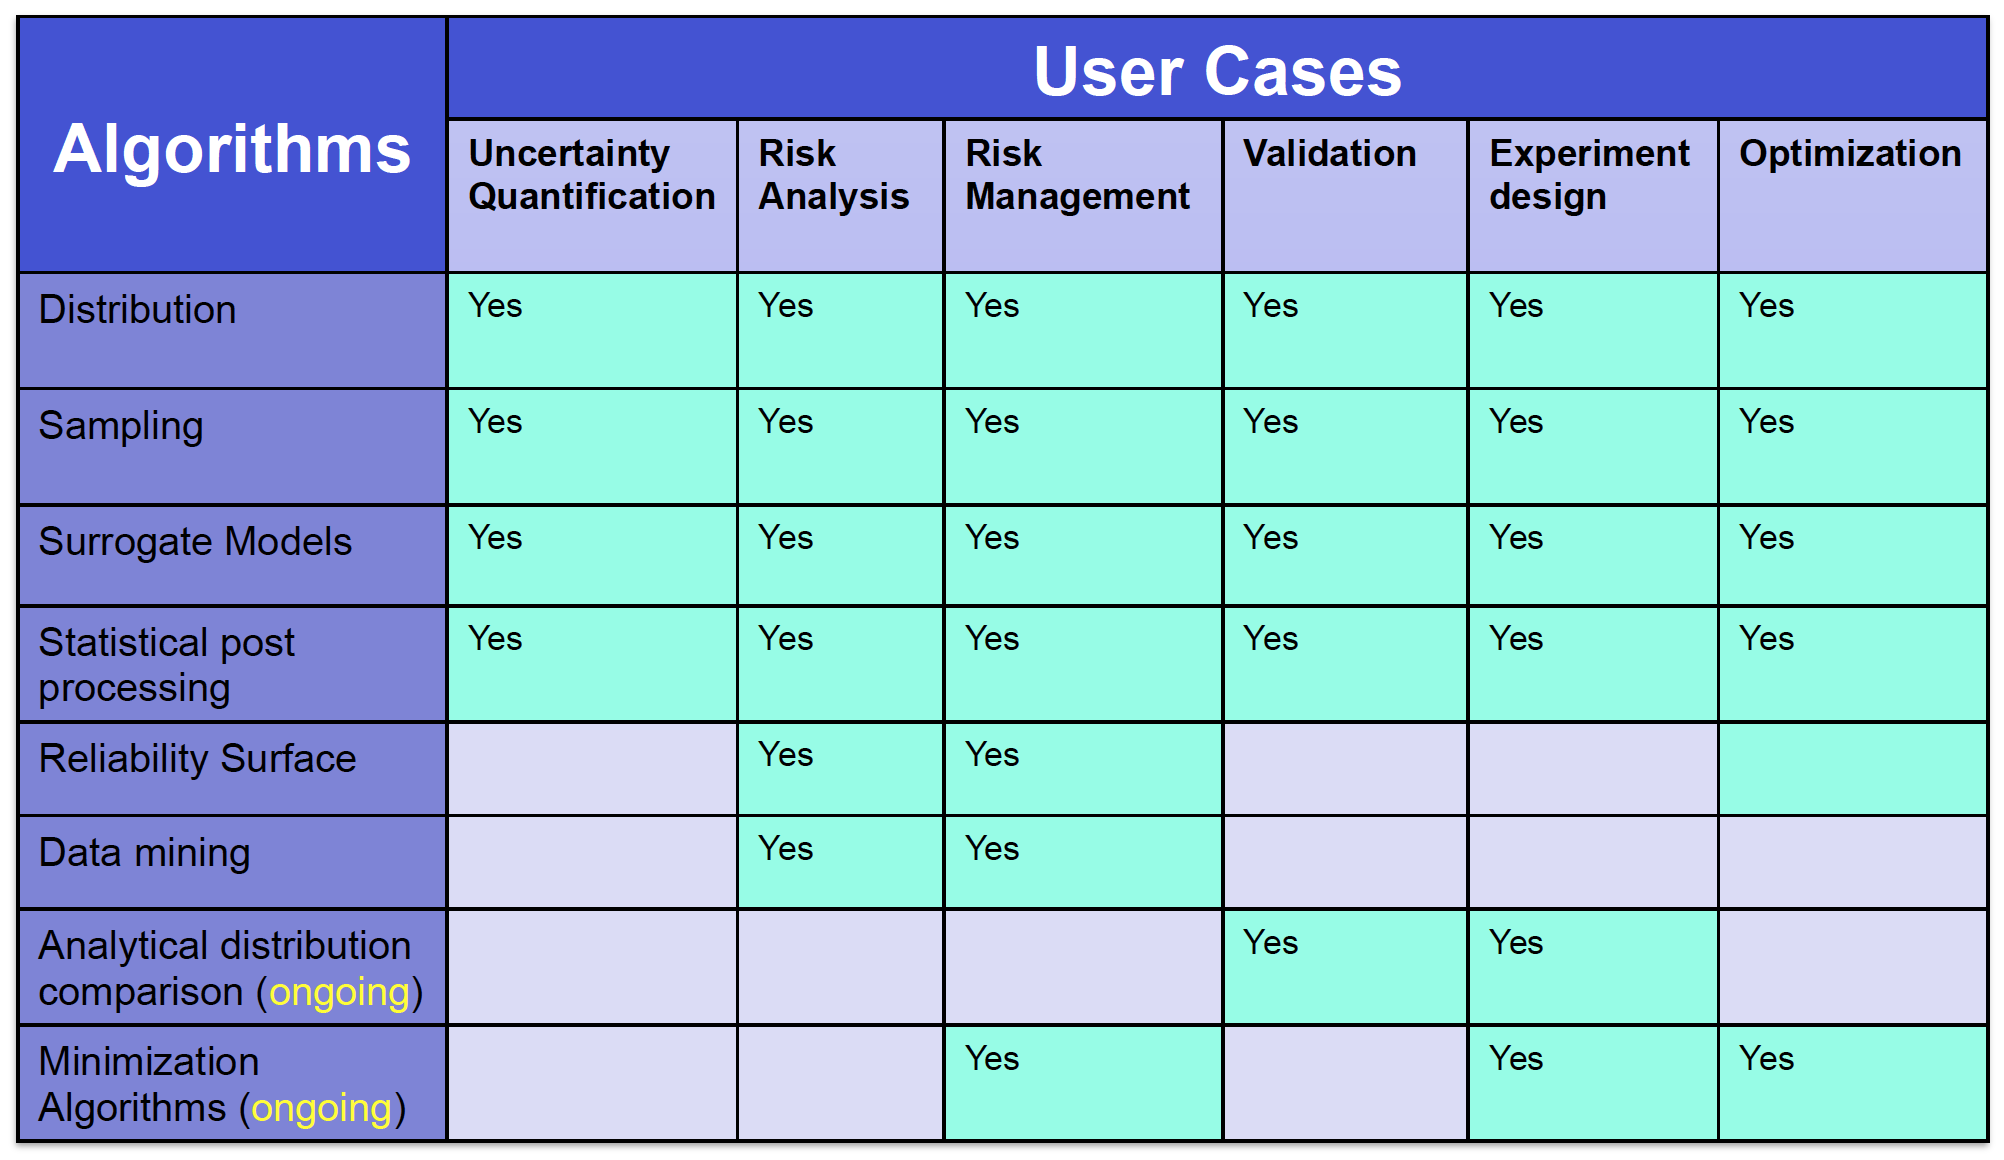
\includegraphics[width=\textwidth]{pics/raven_cap.png}
  \caption{RAVEN Capabilities vs. Needs}
  \label{fig:ravenCap}
\end{figure}

\begin{itemize}
  \item \textbf{Sensitivity Analysis and Uncertainty Quantification}: Sensitivity analysis is a mathematical tool
    that can be used to identify the key sources of uncertainties. Uncertainty quantification is a process by which
    probabilistic information about system responses can be computed according to specified input parameter probability
    distributions. Available approaches in RAVEN include \textbf{Monte Carlo}, \textbf{Grid}, \textbf{Stratified (Latin hypercube)},
    \textbf{Sparse Grid Collocation}, \textbf{Sobol}, \textbf{Adaptive Sparse Grid}, \textbf{Adaptive Sobol} and
    \textbf{BasicStatistics}.
  \item \textbf{Design of Experiments}: The design of experiments (DOE) is a powerful tool that can be used to explore the
    parameter space at a variety of experimental situations. It can be used to determine the relationship between
    input factors and the desired outputs. Available approaches in RAVEN include \textbf{Factorial Design}
    (i.e. General full factorial, 2-level fractional-factorial and Plackett-Burman) and \textbf{Response Surface Design}
    (i.e. Box-Behnken and Central composite algorithms).
  \item \textbf{Risk Mitigation or Model Optimization}: RAVEN uses the \textbf{Optimizer}, a powerful sampler-like entity that searches
    the input space to find minimum or maximum values of a reponse. Currently available optimizers include
    \textbf{Simultaneous Perturbation Stochastic Approximation (SPSA)}.
  \item \textbf{Risk Analysis}: Available approaches in RAVEN include \textbf{Dynamic Event Tree}, \textbf{Limit Surface Search},
    \textbf{Hybrid Dynamic Event Tree}, \textbf{Adaptive Dynamic Event Tree}, \textbf{Adaptive Hybrid Dynamic Event Tree},
    \textbf{Data Mining}, \textbf{Importance Rank}, \textbf{Safest Point}, and \textbf{Basic Statistics}.
  \item \textbf{Risk Management}: Available approaches in RAVEN include \textbf{Reduced order models},
    approaches used for sensitivity and uncertainty analysis, and \textbf{Dynamic Event Tree} methods.
  \item \textbf{Validation}: Available approaches in RAVEN include \textbf{ROMs}, \textbf{Comparison Statistics} and \textbf{Validation Metrics} 
\end{itemize}

In addition, RAVEN includes a number of related advanced capabilities. \textbf{Surrogate or Reduced order models (ROMs)} are mathematical
model trained to predict a response of interest of a physical system. Typically, ROMs trade speed for accuracy representing
a faster, rough estimate of the underlying systems. They can be used to explore the input parameter space for optimization
or sensitivity and uncertainty studies. \textbf{Ensemble Model} is able to combine \textbf{Codes}, \textbf{External Models}
and \textbf{ROMs}. It is intended to create a chain of models whose execution order is determined by the input/output
relationships among them. If the relationships among the models evolve in a non-linear system, a Picard's iteration scheme is
employed.

\subsection{Components of RAVEN}
\label{sub:InputComponents}
The RAVEN code does not have a fixed calculation flow, since all of its basic
objects can be combined in order to create a user-defined calculation flow.
%
Thus, its input, eXtensible Markup Language (XML) format, is organized in different XML blocks, each with a
different functionality. For more information about XML, please click on the link:
\href{https://www.w3schools.com/xml/default.asp}{\textbf{XML tutorial}}.
%
\\The main input blocks are as follows:
\begin{itemize}
  \item \xmlNode{Simulation}: The root node containing the
  entire input, all of
  the following blocks fit inside the \emph{Simulation} block.
  %
  \item \xmlNode{RunInfo}: Specifies the calculation
  settings (number of parallel simulations, etc.).
  %
  \item \xmlNode{Files}: Specifies the files to be
  used in the calculation.
  %
  \item \xmlNode{Distributions}: Defines distributions
  needed for describing parameters, etc.
  %
  \item \xmlNode{Samplers}: Sets up the strategies used for
  exploring an uncertain domain.
  %
  \item \xmlNode{DataObjects}: Specifies internal data objects
  used by RAVEN.
  %
  \item \xmlNode{Databases}: Lists the HDF5 databases used
  as input/output to a
  RAVEN run.
  %
  \item \xmlNode{OutStreams}: Visualization and
  Printing system block.
  %
  \item \xmlNode{Models}: Specifies codes, ROMs,
  post-processing analysis, etc.
  %
  \item \xmlNode{Functions}: Details interfaces to external
  user-defined functions and modules the user will be building and/or running.
  %
  \item \xmlNode{VariableGroups}: Creates a collection of variables.
  %
  \item \xmlNode{Optimizers}: Performs the driving of a specific goal function over
  the model for value optimization.
  %
  \item \xmlNode{Metrics}: Calculate the distance values among points and histories.
  %
  \item \xmlNode{Steps}: Combines other blocks to detail a
  step in the RAVEN workflow including I/O and computations to be performed.
  %
\end{itemize}

Each of these components are explained in dedicated sections of the user manual ~\cite{RAVENuserManual}, and can
be used as building blocks to construct certain calculation flow, as shown in Figure.~\ref{fig:ravenStructure}.
In this guide, we will only show how to use these components to build the analysis flow, and we recommend the user
to check the user manual ~\cite{RAVENuserManual} for the detailed descriptions.

\begin{figure}[h!]
  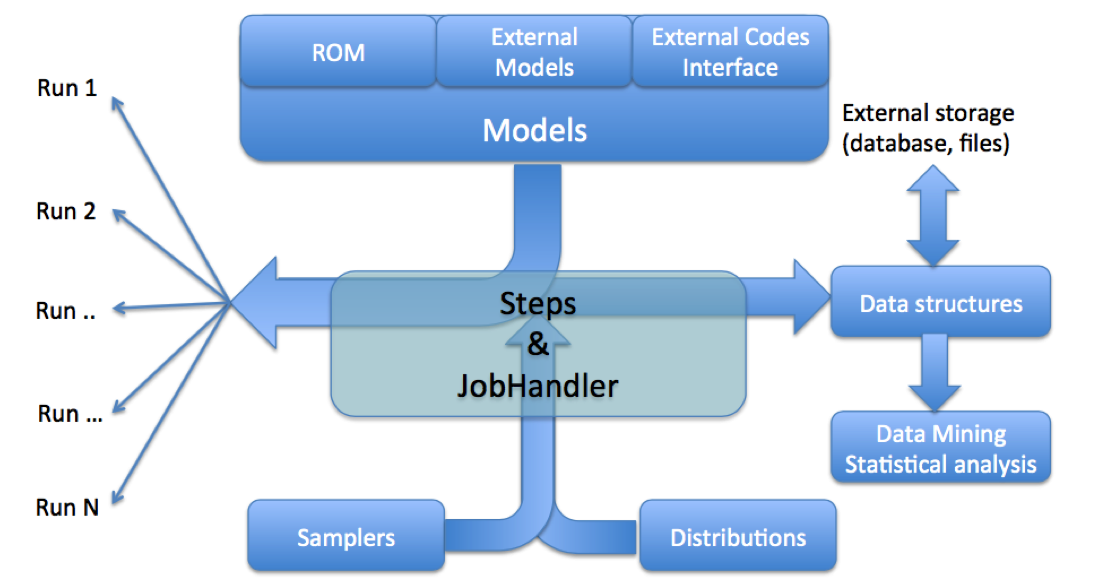
\includegraphics[width=\textwidth]{pics/ravenStructure.png}
  \caption{RAVEN structures}
  \label{fig:ravenStructure}
\end{figure}

In addition, RAVEN allows the user to load any external input file that contains the required XML nodes into the RAVEN main input
file, and provide the standard XML comments, using\verb|<!--| and \verb|-->|. For example, one can use the following template to load
the \xmlNode{Distributions} from file `Distributions.xml'.
%
\begin{lstlisting}[style=XML,morekeywords={node,xmlToLoad}]
<Simulation verbosity='all'>
  ...
  <!-- An Example Comment -->
  <Steps verbosity='debug'>
    ...
  </Steps>
  ...
  <ExternalXML node='Distributions' xmlToLoad='path_to_folder/Distributions.xml'/>
  ...
</Simulation>
\end{lstlisting}
%
RAVEN also allows the user to control the level of output to the user interface by using \xmlAttr{verbosity} system. These settings can be
declared globally as attributes in the \xmlNode{Simulation} node, or locally in each block node as shown in above template.
The verbosity levels are
\begin{itemize}
\item \xmlString{silent} - Only simulation-breaking errors are displayed.
\item \xmlString{quiet} - Errors as well as warnings are displayed.
\item \xmlString{all} (default) - Errors, warnings, and messages are displayed.
\item \xmlString{debug} - For developers. All errors, warnings, messages, and debug messages are displayed.
\end{itemize}



\subsection{Code Interfaces of RAVEN}
The procedure of coupling a new code/application with RAVEN is a straightforward process. The provided Application
Programming Interfaces (APIs) allow RAVEN to interact with any code as long as all the parameters that need to be
perturbed are accessible by input files or via python interfaces. For example, for all the codes currently
supported by RAVEN (e.g. RELAP-7, RELAP-5D, BISON, MAMMOTH, etc.), the coupling is performed through a Python interface
that interprets the information coming from RAVEN and translates them into the input of the driven code. The couping procedure
does not require modifying RAVEN itself. Instread, the developer creates a new Python interface that is going to
be embedded in RAVEN at run-time (no need to introduce hard-coded coupling statements). In addition, RAVEN will
manage concurrent executions of your simulations in parallel, whether on a local desktop or remote high-performance cluster.

Figure.~\ref{fig:modelAPIs} depicts the different APIs between RAVEN and the computational models, i.e. the
\textbf{ROM}, \textbf{External Models} and \textbf{External Code} APIs. 

\begin{figure}[h!]
  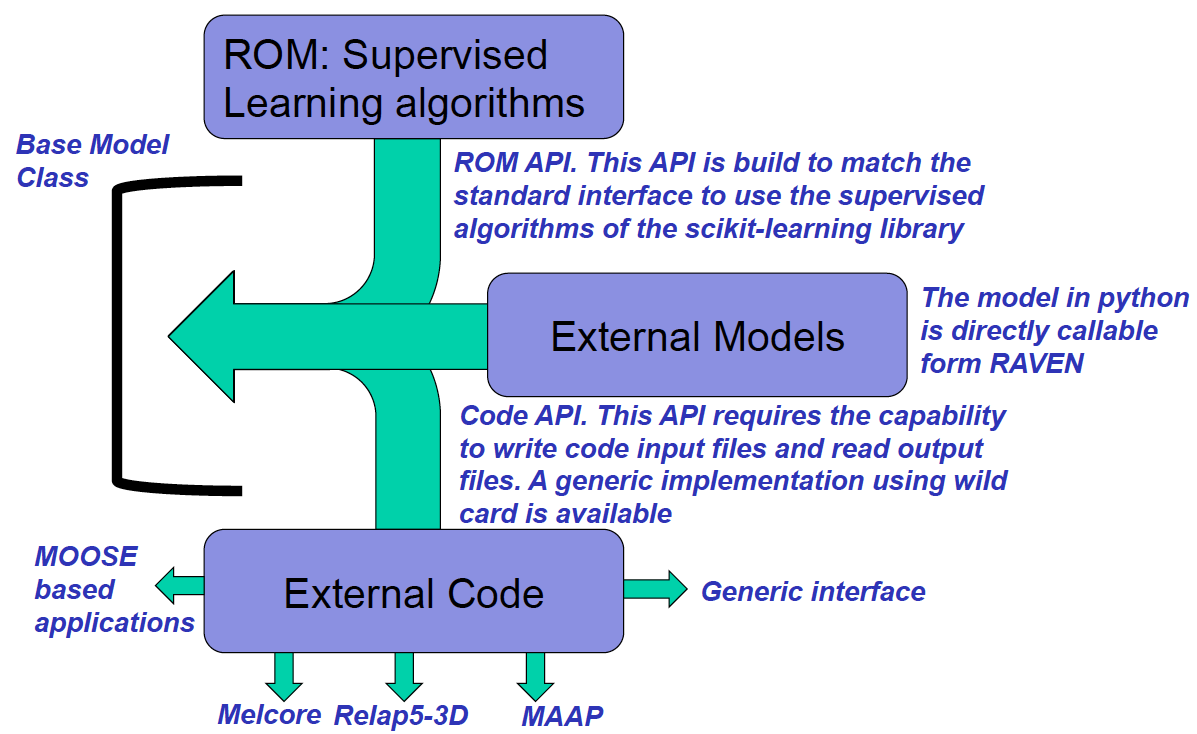
\includegraphics[width=\textwidth]{pics/modelAPIs.png}
  \caption{RAVEN Application Programming Interfaces}
  \label{fig:modelAPIs}
\end{figure}

\clearpage

\subsection{User Guide Organization}
The goal of this document is to provide a set of detailed examples that can help the user to become familiar with
the RAVEN code. RAVEN is capable of investigating system response and explore input space using various
sampling schemes such as Monte Carlo, grid, or Latin Hypercube. However, RAVEN strength lies in its system feature
discovery capabilities such as: constructing limit surfaces, separating regions of the input space leading to
system failure, and using dynamic supervised learning techniques. New users should consult the \textbf{RAVEN Tutorial}
to get started.

\begin{itemize}
  \item \textbf{RAVEN Tutorial}: section~\ref{sec:ravenTutorial}
  \item \textbf{Sampling Strategies}: section~\ref{sec:forwardSamplingStrategies} and section~\ref{sec:adaptiveSamplingStrategies}
  \item \textbf{Restart}: section~\ref{sec:samplingFromRestart}
  \item \textbf{Reduced Order Modeling}: section~\ref{sec:ROMraven}
  \item \textbf{Risk Analysis}: section~\ref{sec:SAraven}
  \item \textbf{Data Mining}: section~\ref{sec:DMraven}
  \item \textbf{Model Optimization}: section~\ref{sec:optimizerStrategies}
  %%%% We may need to add the following sections
  %\item \textbf{Sensitivity Analysis and Uncertainty Quantification}:
  %\item \textbf{Design of Experiments}:
  %\item \textbf{Validation}:
  %\item \textbf{Code Interface}:
  %\item \textbf{Advanced Topics}:
  %  \begin{itemize}
  %    \item Ensemble Forward Sampler:
  %    \item Ensemble Model:
  %  \end{itemize}
\end{itemize}



